\section{Interrupts}
\subsection*{What is an interrupt? }
\begin{frame}
    \frametitle{What is an Interrupt? }
    \begin{figure}
        \includegraphics[height=0.4\textheight]{fig/interrupt.pdf}
        \caption{Interrupt}
    \end{figure}
\end{frame}

\subsection*{Nested interrupts}
\begin{frame}
    \frametitle{Nested interrupts}
    \begin{figure}
        \includegraphics[height=0.4\textheight]{fig/interrupt_nested.pdf}
        \caption{nested interrupt}
    \end{figure}
\end{frame}

\subsection*{Reentrancy}
\begin{frame}
    \frametitle{Reentrancy}
    \begin{figure}
        \includegraphics[height=0.4\textheight]{fig/interrupt_reentrancy.pdf}
        \caption{Non reentrant function f()}
    \end{figure}
\end{frame}

